\documentclass[journal,12pt,twocolumn]{IEEEtran}
%
\usepackage[latin1]{inputenc}
\usepackage{setspace}
\usepackage{gensymb}
\doublespacing
\singlespacing

\usepackage{graphicx}
\usepackage{amssymb}
%\usepackage{relsize}
\usepackage[cmex10]{amsmath}
\usepackage{amsthm}
%\interdisplaylinepenalty=2500
%\savesymbol{iint}
%\usepackage{txfonts}
%\restoresymbol{TXF}{iint}
%\usepackage{wasysym}
\usepackage{amsthm}
%\usepackage{iithtlc}
\usepackage{mathrsfs}
\usepackage{txfonts}
\usepackage{stfloats}
\usepackage{bm}
\usepackage{cite}
\usepackage{cases}
\usepackage{subfig}
%\usepackage{xtab}
\usepackage{longtable}
\usepackage{multirow}
%\usepackage{algorithm}
%\usepackage{algpseudocode}
\usepackage{enumitem}
\usepackage{mathtools}
\usepackage{steinmetz}
\usepackage{tikz}
\usepackage{circuitikz}
\usepackage{verbatim}
\usepackage{tfrupee}
\usepackage[breaklinks=true]{hyperref}
%\usepackage{stmaryrd}
\usepackage{tkz-euclide} % loads  TikZ and tkz-base
%\usetkzobj{all}
\usetikzlibrary{calc,math}
\usepackage{listings}
    \usepackage{color}                                            %%
    \usepackage{array}                                            %%
    \usepackage{longtable}                                        %%
    \usepackage{calc}                                             %%
    \usepackage{multirow}                                         %%
    \usepackage{hhline}                                           %%
    \usepackage{ifthen}                                           %%
  %optionally (for landscape tables embedded in another document): %%
    \usepackage{lscape}     
\usepackage{multicol}
\usepackage{chngcntr}
%\usepackage{enumerate}
\usepackage{graphics}
%\usepackage{wasysym}
%\newcounter{MYtempeqncnt}
\DeclareMathOperator*{\Res}{Res}
%\renewcommand{\baselinestretch}{2}
\renewcommand\thesection{\arabic{section}}
\renewcommand\thesubsection{\thesection.\arabic{subsection}}
\renewcommand\thesubsubsection{\thesubsection.\arabic{subsubsection}}
\renewcommand{\theequation}{\thesection\arabic{equation}}
\renewcommand\thesectiondis{\arabic{section}}
\renewcommand\thesubsectiondis{\thesectiondis.\arabic{subsection}}
\renewcommand\thesubsubsectiondis{\thesubsectiondis.\arabic{subsubsection}}

% correct bad hyphenation here
\hyphenation{op-tical net-works semi-conduc-tor}
\def\inputGnumericTable{}                                 %%

\lstset{
%language=C,
frame=single, 
breaklines=true,
columns=fullflexible
}
%\lstset{
%language=tex,
%frame=single, 
%breaklines=true
%}

\begin{document}
%


\newtheorem{theorem}{Theorem}[section]
\newtheorem{problem}{Problem}
\newtheorem{proposition}{Proposition}[section]
\newtheorem{lemma}{Lemma}[section]
\newtheorem{corollary}[theorem]{Corollary}
\newtheorem{example}{Example}[section]
\newtheorem{definition}[problem]{Definition}
%\newtheorem{thm}{Theorem}[section] 
%\newtheorem{defn}[thm]{Definition}
%\newtheorem{algorithm}{Algorithm}[section]
%\newtheorem{cor}{Corollary}
\newcommand{\BEQA}{\begin{eqnarray}}
\newcommand{\EEQA}{\end{eqnarray}}
\newcommand{\define}{\stackrel{\triangle}{=}}
\bibliographystyle{IEEEtran}
%\bibliographystyle{ieeetr}
\providecommand{\mbf}{\mathbf}
\providecommand{\pr}[1]{\ensuremath{\Pr\left(#1\right)}}
\providecommand{\qfunc}[1]{\ensuremath{Q\left(#1\right)}}
\providecommand{\sbrak}[1]{\ensuremath{{}\left[#1\right]}}
\providecommand{\lsbrak}[1]{\ensuremath{{}\left[#1\right.}}
\providecommand{\rsbrak}[1]{\ensuremath{{}\left.#1\right]}}
\providecommand{\brak}[1]{\ensuremath{\left(#1\right)}}
\providecommand{\lbrak}[1]{\ensuremath{\left(#1\right.}}
\providecommand{\rbrak}[1]{\ensuremath{\left.#1\right)}}
\providecommand{\cbrak}[1]{\ensuremath{\left\{#1\right\}}}
\providecommand{\lcbrak}[1]{\ensuremath{\left\{#1\right.}}
\providecommand{\rcbrak}[1]{\ensuremath{\left.#1\right\}}}
\theoremstyle{remark}
\newtheorem{rem}{Remark}
\newcommand{\sgn}{\mathop{\mathrm{sgn}}}
\providecommand{\abs}[1]{\left\vert#1\right\vert}
\providecommand{\res}[1]{\Res\displaylimits_{#1}} 
\providecommand{\norm}[1]{\left\lVert#1\right\rVert}
%\providecommand{\norm}[1]{\lVert#1\rVert}
\providecommand{\mtx}[1]{\mathbf{#1}}
\providecommand{\mean}[1]{E\left[ #1 \right]}
\providecommand{\fourier}{\overset{\mathcal{F}}{ \rightleftharpoons}}
%\providecommand{\hilbert}{\overset{\mathcal{H}}{ \rightleftharpoons}}
\providecommand{\system}{\overset{\mathcal{H}}{ \longleftrightarrow}}
	%\newcommand{\solution}[2]{\textbf{Solution:}{#1}}
\newcommand{\solution}{\noindent \textbf{Solution: }}
\newcommand{\cosec}{\,\text{cosec}\,}
\providecommand{\dec}[2]{\ensuremath{\overset{#1}{\underset{#2}{\gtrless}}}}
\newcommand{\myvec}[1]{\ensuremath{\begin{pmatrix}#1\end{pmatrix}}}
\newcommand{\mydet}[1]{\ensuremath{\begin{vmatrix}#1\end{vmatrix}}}
%\numberwithin{equation}{section}
\numberwithin{equation}{subsection}
%\numberwithin{problem}{section}
%\numberwithin{definition}{section}
\makeatletter
\@addtoreset{figure}{problem}
\makeatother
\let\StandardTheFigure\thefigure
\let\vec\mathbf
%\renewcommand{\thefigure}{\theproblem.\arabic{figure}}
%\renewcommand{\thefigure}{\theproblem}
%\setlist[enumerate,1]{before=\renewcommand\theequation{\theenumi.\arabic{equation}}
%\counterwithin{equation}{enumi}
%\renewcommand{\theequation}{\arabic{subsection}.\arabic{equation}}
\def\putbox#1#2#3{\makebox[0in][l]{\makebox[#1][l]{}\raisebox{\baselineskip}[0in][0in]{\raisebox{#2}[0in][0in]{#3}}}}
     \def\rightbox#1{\makebox[0in][r]{#1}}
     \def\centbox#1{\makebox[0in]{#1}}
     \def\topbox#1{\raisebox{-\baselineskip}[0in][0in]{#1}}
     \def\midbox#1{\raisebox{-0.5\baselineskip}[0in][0in]{#1}}
\vspace{3cm}
\title{Linear Algebra}
\author{Mohit Singh}

\maketitle{}
\newpage
%\tableofcontents
\bigskip
\renewcommand{\thefigure}{\theenumi}
\renewcommand{\thetable}{\theenumi}

\begin{abstract}
This document provides the solution to the problem no. 7 of each section under  linear algebra. The figures are constructed using python.
\end{abstract}

\noindent This documentation can be downloaded from 
%
\begin{lstlisting}
svn co https://github.com/mohit-singh-9/Summer-2020/tree/master/geometry/linear_algebra.git
\end{lstlisting}
%
%and latex-tikz codes from 
%\begin{lstlisting}
%math/codes/tri_sss.py
%\end{lstlisting}

\section{TRIANGLE EXERCISE}
\subsection{Problem}
\begin{flushleft}
Find the center and radius of the circle
\begin{align}
\vec{x}^T\vec{x} + \myvec{8\\10}\vec{x} - 8 = 0
\end{align}
\end{flushleft}

\subsection{Solution}
The given curve 
\begin{align}
	y =\frac{1}{x-1}
\end{align}
can be expressed as 
\begin{align}
	xy - y - 1 = 0 \label{eq:solutions/1/14/eq:hyperbola}
\end{align}
Hence, we have
\begin{align}
	\vec{V} = \frac{1}{2}\myvec{0 & 1 \\ 1 & 0}, 
	\vec{u} = \frac{1}{2}\myvec{0 \\-1},
	f = -1
\end{align}
Since $\mydet{\vec{V}} < 0$, the equation \eqref{eq:solutions/1/14/eq:hyperbola} represents hyperbola.
To find the values of $\lambda_1$ and $\lambda_2$, consider the characteristic equation,
\begin{align}
	\mydet{\lambda\vec{I} - \vec{V}} &= 0\\
	\implies \mydet{\myvec{\lambda & 0\\0 & \lambda} - \myvec{0 & \frac{1}{2} \\ \frac{1}{2} & 0}} &= 0\\
	\implies \mydet{ \lambda & \frac{-1}{2} \\ \frac{-1}{2} & \lambda} &= 0\\
	\implies \lambda_1 &= \frac{1}{2} , \lambda_2 = \frac{-1}{2}
\end{align}
In addition, given the slope -1, the direction and normal vectors are given by 
\begin{align}
	\vec{m} = \myvec{1 \\ -1} \\
	\vec{n} = \myvec{ 1 \\ 1}
\end{align}
The parameters of hyperbola are as follows:
\begin{align}
	\vec{c} &= -\vec{V}^{-1}\vec{u} \\
	&= -\myvec{0 & 2\\ 2 & 0}\myvec{0 \\ -\frac{1}{2}} \\
	&= \myvec{1 \\ 0}\\
	axes &= \begin{cases}
	\sqrt{\frac{\vec{u}^T\vec{V}^{-1}\vec{u} - f}{\lambda_1}} = \sqrt{2}\\
 \sqrt{\frac{f-\vec{u}^T\vec{V}^{-1}\vec{u}}{\lambda_2}} = \sqrt{2}
\end{cases}
\end{align}
which represents the standard hyperbola equation,
\begin{align}
	\frac{x^2}{2} - \frac{x^2}{2} = 1
\end{align}
The points of contact are given by 
\begin{align}
  \tiny{K} &=\pm \sqrt{\frac{\vec{u}^T\vec{V}^{-1}\vec{u} - f}{\vec{n}^T\vec{V}^{-1}\vec{n}}}
  = \pm \frac{1}{2}\\
  \vec{q} &= \vec{V}^{-1}(k\vec{n}-\vec{u})\\
  \vec{q_1} &= \myvec{0 & 2\\2 & 0} \sbrak{\frac{1}{2}\myvec{1 \\ 1} - \myvec{0\\ \frac{-1}{2}}}\\
  &= \myvec{2 \\ 1}\\
  \vec{q_2} &= \myvec{0 & 2\\2 & 0} \sbrak{\frac{-1}{2}\myvec{1 \\ 1} - \myvec{0\\ \frac{-1}{2}}}\\
  &= \myvec{0 \\ -1}
\end{align} 
$\therefore$ The tangents are given by
\begin{align}
	\myvec{1 & 1} \brak{\vec{x} - \myvec{2 \\ 1}} = 0 \\
	\myvec{1 & 1} \brak{\vec{x} - \myvec{0 \\ -1}} = 0
\end{align}
The desired equations of all lines having slope -1 that are tangents to the curve $\frac{1}{x-1}, x \neq 1$ are given by
\begin{align}
	\myvec{1 & 1}\vec{x} &= 3 \\
	\myvec{1 & 1}\vec{x} &= -1 
\end{align}
The above results are verified in the following figure.
\begin{figure}[h!] \label{eq:solutions/1/14/fig:tangents}
	\centering
	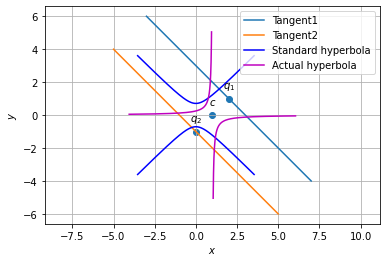
\includegraphics[width=\columnwidth]{./solutions/1/14/graph7.png}
	\caption{The standard and actual hyperbola.}
\end{figure}


\section{QUADRILATERAL EXERCISE}
\subsection{Problem}
\begin{flushleft}
Find the center and radius of the circle
\begin{align}
\vec{x}^T\vec{x} + \myvec{8\\10}\vec{x} - 8 = 0
\end{align}
\end{flushleft}

\subsection{Solution}
\begin{figure}[!ht]
\centering
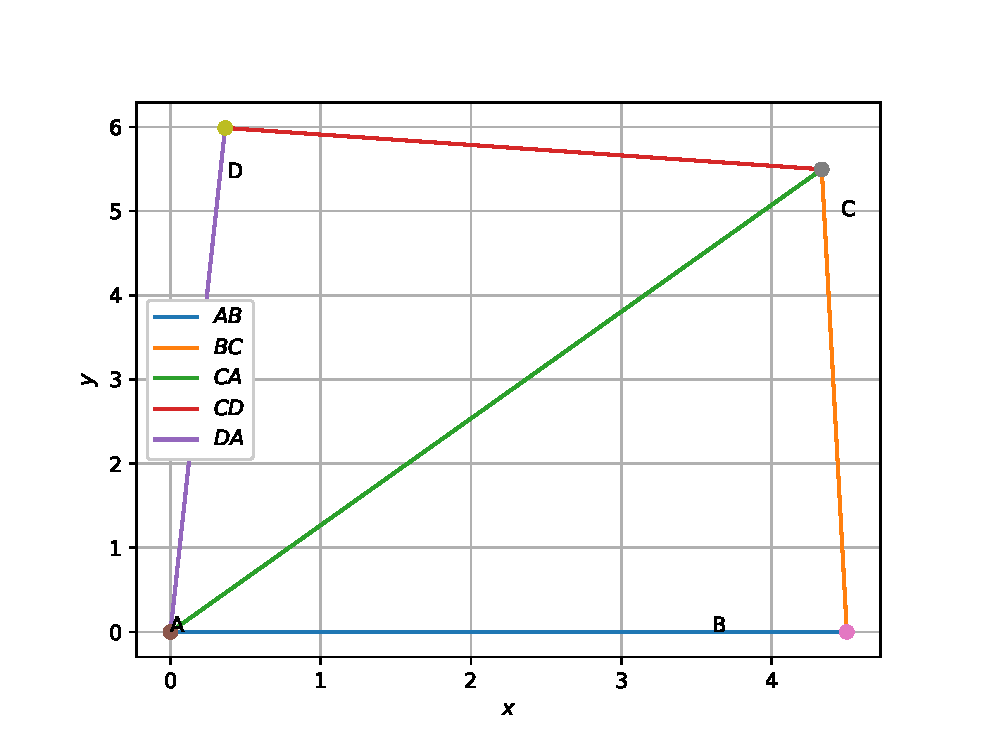
\includegraphics[width= \columnwidth]{./solutions/7/figs/quad/quad.eps}
\caption{Square ABCD}
\label{fig:2.2.7}
\end{figure}
See Fig. \ref{fig:2.2.7}.

\begin{enumerate}
\item From inspection we see that the opposite vertices forms a diagonal which is parallel to x-axis. Then the diagonal formed by other two vertices is parallel to y-axis(i.e. their x coordinates are equal). Let $\vec{A}= \myvec{-1\\2}$  and $\vec{C}=\myvec{3\\2}$. 

\item Diagonals bisect each other at 90\degree.
Let $\vec{B}$ and $\vec{D}$ be other two vertices. 
\item Using the property that diagonals bisect each other at 90\degree, we can obtain other vertices by rotating diagonal AC by 90\degree about $\vec{E}$ in clockwise or anticlockwise direction.

\item The rotation matrix for a rotation of angle 90\degree about origin in anticlockwise direction is given by
\begin{align}
\myvec{\cos90\degree&-\sin90\degree\\\sin90\degree&\cos90\degree}=\myvec{0&-1\\1&0}
\end{align}
The $\vec{E}$ is given by
\begin{align}
\vec{E}&= \frac{\vec{A}+\vec{C}}{2} \\
&= \myvec{1\\2}
\end{align}

\item To make the rotation we need to shift the $\vec{E}$ to origin. So the change in other vectors are
\begin{align}
\vec{A}-\vec{E}&=\myvec{-2\\0}\\
\vec{C}-\vec{E}&=\myvec{2\\0}
\end{align}

The required matrix now is $\myvec{-2&2\\0&0}$. Multiplying this with rotation matrix 
\begin{align}
&= \myvec{0&-1\\1&0}\myvec{-2&2\\0&0}\\
&=\myvec{0&0\\-2&2}
\end{align}
Now we obtained the coordinates as $\myvec{0\\-2}$ and $\myvec{0\\2}$.
To obtain the final coordinates we will add $\vec{E}$ to shift to the actual position.
\begin{align}
\vec{B}=\myvec{0\\-2}+\myvec{1\\2}\\
\vec{D}=\myvec{0\\2}+\myvec{1\\2}
\end{align}
Thus 
\begin{align}
\vec{B}&= \myvec{1\\0} \\
\vec{D}&= \myvec{1\\4}
\end{align} 
\item The python code for the figure can be downloaded from
\begin{lstlisting}
solutions/7/codes/quad/quad.py
\end{lstlisting}
\end{enumerate}  



\section{LINE EXERCISE}
\subsection{Matrix}
\subsubsection{Problem}
\begin{flushleft}
Find the center and radius of the circle
\begin{align}
\vec{x}^T\vec{x} + \myvec{8\\10}\vec{x} - 8 = 0
\end{align}
\end{flushleft}

\subsubsection{Solution}
The given curve 
\begin{align}
	y =\frac{1}{x-1}
\end{align}
can be expressed as 
\begin{align}
	xy - y - 1 = 0 \label{eq:solutions/1/14/eq:hyperbola}
\end{align}
Hence, we have
\begin{align}
	\vec{V} = \frac{1}{2}\myvec{0 & 1 \\ 1 & 0}, 
	\vec{u} = \frac{1}{2}\myvec{0 \\-1},
	f = -1
\end{align}
Since $\mydet{\vec{V}} < 0$, the equation \eqref{eq:solutions/1/14/eq:hyperbola} represents hyperbola.
To find the values of $\lambda_1$ and $\lambda_2$, consider the characteristic equation,
\begin{align}
	\mydet{\lambda\vec{I} - \vec{V}} &= 0\\
	\implies \mydet{\myvec{\lambda & 0\\0 & \lambda} - \myvec{0 & \frac{1}{2} \\ \frac{1}{2} & 0}} &= 0\\
	\implies \mydet{ \lambda & \frac{-1}{2} \\ \frac{-1}{2} & \lambda} &= 0\\
	\implies \lambda_1 &= \frac{1}{2} , \lambda_2 = \frac{-1}{2}
\end{align}
In addition, given the slope -1, the direction and normal vectors are given by 
\begin{align}
	\vec{m} = \myvec{1 \\ -1} \\
	\vec{n} = \myvec{ 1 \\ 1}
\end{align}
The parameters of hyperbola are as follows:
\begin{align}
	\vec{c} &= -\vec{V}^{-1}\vec{u} \\
	&= -\myvec{0 & 2\\ 2 & 0}\myvec{0 \\ -\frac{1}{2}} \\
	&= \myvec{1 \\ 0}\\
	axes &= \begin{cases}
	\sqrt{\frac{\vec{u}^T\vec{V}^{-1}\vec{u} - f}{\lambda_1}} = \sqrt{2}\\
 \sqrt{\frac{f-\vec{u}^T\vec{V}^{-1}\vec{u}}{\lambda_2}} = \sqrt{2}
\end{cases}
\end{align}
which represents the standard hyperbola equation,
\begin{align}
	\frac{x^2}{2} - \frac{x^2}{2} = 1
\end{align}
The points of contact are given by 
\begin{align}
  \tiny{K} &=\pm \sqrt{\frac{\vec{u}^T\vec{V}^{-1}\vec{u} - f}{\vec{n}^T\vec{V}^{-1}\vec{n}}}
  = \pm \frac{1}{2}\\
  \vec{q} &= \vec{V}^{-1}(k\vec{n}-\vec{u})\\
  \vec{q_1} &= \myvec{0 & 2\\2 & 0} \sbrak{\frac{1}{2}\myvec{1 \\ 1} - \myvec{0\\ \frac{-1}{2}}}\\
  &= \myvec{2 \\ 1}\\
  \vec{q_2} &= \myvec{0 & 2\\2 & 0} \sbrak{\frac{-1}{2}\myvec{1 \\ 1} - \myvec{0\\ \frac{-1}{2}}}\\
  &= \myvec{0 \\ -1}
\end{align} 
$\therefore$ The tangents are given by
\begin{align}
	\myvec{1 & 1} \brak{\vec{x} - \myvec{2 \\ 1}} = 0 \\
	\myvec{1 & 1} \brak{\vec{x} - \myvec{0 \\ -1}} = 0
\end{align}
The desired equations of all lines having slope -1 that are tangents to the curve $\frac{1}{x-1}, x \neq 1$ are given by
\begin{align}
	\myvec{1 & 1}\vec{x} &= 3 \\
	\myvec{1 & 1}\vec{x} &= -1 
\end{align}
The above results are verified in the following figure.
\begin{figure}[h!] \label{eq:solutions/1/14/fig:tangents}
	\centering
	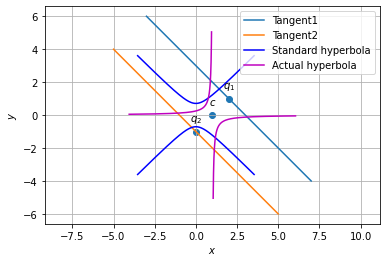
\includegraphics[width=\columnwidth]{./solutions/1/14/graph7.png}
	\caption{The standard and actual hyperbola.}
\end{figure}


\subsection{Complex Numbers}
\subsubsection{Problem}
\begin{flushleft}
Find the center and radius of the circle
\begin{align}
\vec{x}^T\vec{x} + \myvec{8\\10}\vec{x} - 8 = 0
\end{align}
\end{flushleft}

\subsubsection{Solution}
\begin{figure}[!ht]
\centering
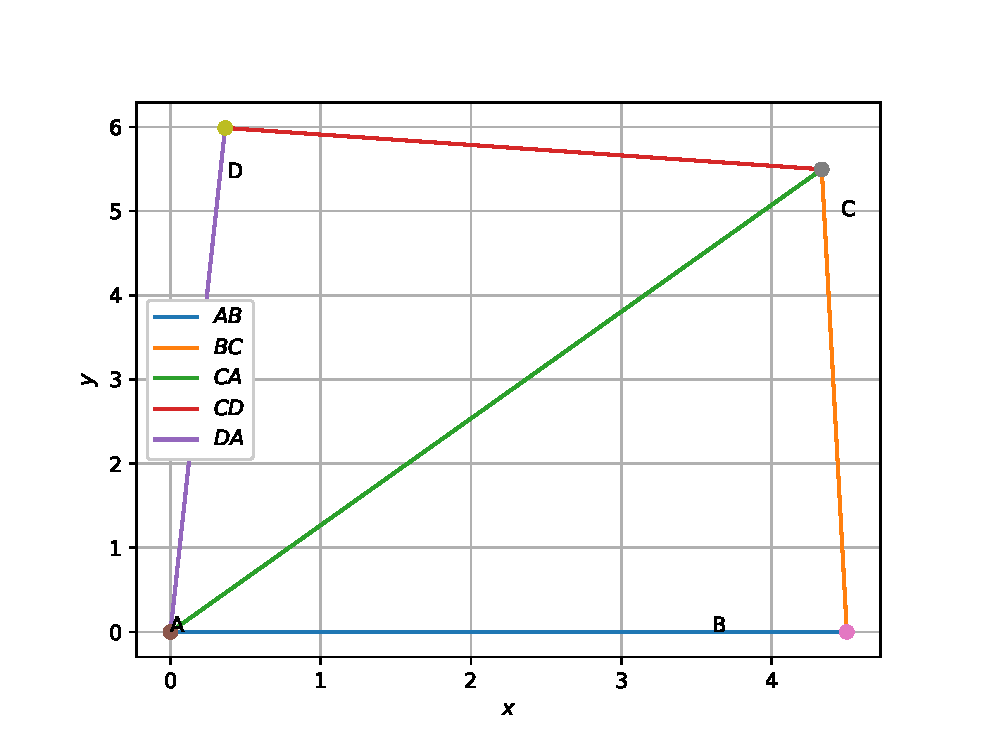
\includegraphics[width= \columnwidth]{./solutions/7/figs/quad/quad.eps}
\caption{Square ABCD}
\label{fig:2.2.7}
\end{figure}
See Fig. \ref{fig:2.2.7}.

\begin{enumerate}
\item From inspection we see that the opposite vertices forms a diagonal which is parallel to x-axis. Then the diagonal formed by other two vertices is parallel to y-axis(i.e. their x coordinates are equal). Let $\vec{A}= \myvec{-1\\2}$  and $\vec{C}=\myvec{3\\2}$. 

\item Diagonals bisect each other at 90\degree.
Let $\vec{B}$ and $\vec{D}$ be other two vertices. 
\item Using the property that diagonals bisect each other at 90\degree, we can obtain other vertices by rotating diagonal AC by 90\degree about $\vec{E}$ in clockwise or anticlockwise direction.

\item The rotation matrix for a rotation of angle 90\degree about origin in anticlockwise direction is given by
\begin{align}
\myvec{\cos90\degree&-\sin90\degree\\\sin90\degree&\cos90\degree}=\myvec{0&-1\\1&0}
\end{align}
The $\vec{E}$ is given by
\begin{align}
\vec{E}&= \frac{\vec{A}+\vec{C}}{2} \\
&= \myvec{1\\2}
\end{align}

\item To make the rotation we need to shift the $\vec{E}$ to origin. So the change in other vectors are
\begin{align}
\vec{A}-\vec{E}&=\myvec{-2\\0}\\
\vec{C}-\vec{E}&=\myvec{2\\0}
\end{align}

The required matrix now is $\myvec{-2&2\\0&0}$. Multiplying this with rotation matrix 
\begin{align}
&= \myvec{0&-1\\1&0}\myvec{-2&2\\0&0}\\
&=\myvec{0&0\\-2&2}
\end{align}
Now we obtained the coordinates as $\myvec{0\\-2}$ and $\myvec{0\\2}$.
To obtain the final coordinates we will add $\vec{E}$ to shift to the actual position.
\begin{align}
\vec{B}=\myvec{0\\-2}+\myvec{1\\2}\\
\vec{D}=\myvec{0\\2}+\myvec{1\\2}
\end{align}
Thus 
\begin{align}
\vec{B}&= \myvec{1\\0} \\
\vec{D}&= \myvec{1\\4}
\end{align} 
\item The python code for the figure can be downloaded from
\begin{lstlisting}
solutions/7/codes/quad/quad.py
\end{lstlisting}
\end{enumerate}  


\subsection{Points and Vectors}
\subsubsection{Problem}
\begin{flushleft}
Find the center and radius of the circle
\begin{align}
\vec{x}^T\vec{x} + \myvec{8\\10}\vec{x} - 8 = 0
\end{align}
\end{flushleft}

\subsubsection{Solution}
The given curve 
\begin{align}
	y =\frac{1}{x-1}
\end{align}
can be expressed as 
\begin{align}
	xy - y - 1 = 0 \label{eq:solutions/1/14/eq:hyperbola}
\end{align}
Hence, we have
\begin{align}
	\vec{V} = \frac{1}{2}\myvec{0 & 1 \\ 1 & 0}, 
	\vec{u} = \frac{1}{2}\myvec{0 \\-1},
	f = -1
\end{align}
Since $\mydet{\vec{V}} < 0$, the equation \eqref{eq:solutions/1/14/eq:hyperbola} represents hyperbola.
To find the values of $\lambda_1$ and $\lambda_2$, consider the characteristic equation,
\begin{align}
	\mydet{\lambda\vec{I} - \vec{V}} &= 0\\
	\implies \mydet{\myvec{\lambda & 0\\0 & \lambda} - \myvec{0 & \frac{1}{2} \\ \frac{1}{2} & 0}} &= 0\\
	\implies \mydet{ \lambda & \frac{-1}{2} \\ \frac{-1}{2} & \lambda} &= 0\\
	\implies \lambda_1 &= \frac{1}{2} , \lambda_2 = \frac{-1}{2}
\end{align}
In addition, given the slope -1, the direction and normal vectors are given by 
\begin{align}
	\vec{m} = \myvec{1 \\ -1} \\
	\vec{n} = \myvec{ 1 \\ 1}
\end{align}
The parameters of hyperbola are as follows:
\begin{align}
	\vec{c} &= -\vec{V}^{-1}\vec{u} \\
	&= -\myvec{0 & 2\\ 2 & 0}\myvec{0 \\ -\frac{1}{2}} \\
	&= \myvec{1 \\ 0}\\
	axes &= \begin{cases}
	\sqrt{\frac{\vec{u}^T\vec{V}^{-1}\vec{u} - f}{\lambda_1}} = \sqrt{2}\\
 \sqrt{\frac{f-\vec{u}^T\vec{V}^{-1}\vec{u}}{\lambda_2}} = \sqrt{2}
\end{cases}
\end{align}
which represents the standard hyperbola equation,
\begin{align}
	\frac{x^2}{2} - \frac{x^2}{2} = 1
\end{align}
The points of contact are given by 
\begin{align}
  \tiny{K} &=\pm \sqrt{\frac{\vec{u}^T\vec{V}^{-1}\vec{u} - f}{\vec{n}^T\vec{V}^{-1}\vec{n}}}
  = \pm \frac{1}{2}\\
  \vec{q} &= \vec{V}^{-1}(k\vec{n}-\vec{u})\\
  \vec{q_1} &= \myvec{0 & 2\\2 & 0} \sbrak{\frac{1}{2}\myvec{1 \\ 1} - \myvec{0\\ \frac{-1}{2}}}\\
  &= \myvec{2 \\ 1}\\
  \vec{q_2} &= \myvec{0 & 2\\2 & 0} \sbrak{\frac{-1}{2}\myvec{1 \\ 1} - \myvec{0\\ \frac{-1}{2}}}\\
  &= \myvec{0 \\ -1}
\end{align} 
$\therefore$ The tangents are given by
\begin{align}
	\myvec{1 & 1} \brak{\vec{x} - \myvec{2 \\ 1}} = 0 \\
	\myvec{1 & 1} \brak{\vec{x} - \myvec{0 \\ -1}} = 0
\end{align}
The desired equations of all lines having slope -1 that are tangents to the curve $\frac{1}{x-1}, x \neq 1$ are given by
\begin{align}
	\myvec{1 & 1}\vec{x} &= 3 \\
	\myvec{1 & 1}\vec{x} &= -1 
\end{align}
The above results are verified in the following figure.
\begin{figure}[h!] \label{eq:solutions/1/14/fig:tangents}
	\centering
	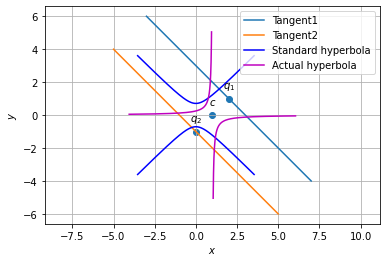
\includegraphics[width=\columnwidth]{./solutions/1/14/graph7.png}
	\caption{The standard and actual hyperbola.}
\end{figure}



\subsection{Points on a Line}
\subsubsection{Problem}
\begin{flushleft}
Find the center and radius of the circle
\begin{align}
\vec{x}^T\vec{x} + \myvec{8\\10}\vec{x} - 8 = 0
\end{align}
\end{flushleft}

\subsubsection{Solution}
The given curve 
\begin{align}
	y =\frac{1}{x-1}
\end{align}
can be expressed as 
\begin{align}
	xy - y - 1 = 0 \label{eq:solutions/1/14/eq:hyperbola}
\end{align}
Hence, we have
\begin{align}
	\vec{V} = \frac{1}{2}\myvec{0 & 1 \\ 1 & 0}, 
	\vec{u} = \frac{1}{2}\myvec{0 \\-1},
	f = -1
\end{align}
Since $\mydet{\vec{V}} < 0$, the equation \eqref{eq:solutions/1/14/eq:hyperbola} represents hyperbola.
To find the values of $\lambda_1$ and $\lambda_2$, consider the characteristic equation,
\begin{align}
	\mydet{\lambda\vec{I} - \vec{V}} &= 0\\
	\implies \mydet{\myvec{\lambda & 0\\0 & \lambda} - \myvec{0 & \frac{1}{2} \\ \frac{1}{2} & 0}} &= 0\\
	\implies \mydet{ \lambda & \frac{-1}{2} \\ \frac{-1}{2} & \lambda} &= 0\\
	\implies \lambda_1 &= \frac{1}{2} , \lambda_2 = \frac{-1}{2}
\end{align}
In addition, given the slope -1, the direction and normal vectors are given by 
\begin{align}
	\vec{m} = \myvec{1 \\ -1} \\
	\vec{n} = \myvec{ 1 \\ 1}
\end{align}
The parameters of hyperbola are as follows:
\begin{align}
	\vec{c} &= -\vec{V}^{-1}\vec{u} \\
	&= -\myvec{0 & 2\\ 2 & 0}\myvec{0 \\ -\frac{1}{2}} \\
	&= \myvec{1 \\ 0}\\
	axes &= \begin{cases}
	\sqrt{\frac{\vec{u}^T\vec{V}^{-1}\vec{u} - f}{\lambda_1}} = \sqrt{2}\\
 \sqrt{\frac{f-\vec{u}^T\vec{V}^{-1}\vec{u}}{\lambda_2}} = \sqrt{2}
\end{cases}
\end{align}
which represents the standard hyperbola equation,
\begin{align}
	\frac{x^2}{2} - \frac{x^2}{2} = 1
\end{align}
The points of contact are given by 
\begin{align}
  \tiny{K} &=\pm \sqrt{\frac{\vec{u}^T\vec{V}^{-1}\vec{u} - f}{\vec{n}^T\vec{V}^{-1}\vec{n}}}
  = \pm \frac{1}{2}\\
  \vec{q} &= \vec{V}^{-1}(k\vec{n}-\vec{u})\\
  \vec{q_1} &= \myvec{0 & 2\\2 & 0} \sbrak{\frac{1}{2}\myvec{1 \\ 1} - \myvec{0\\ \frac{-1}{2}}}\\
  &= \myvec{2 \\ 1}\\
  \vec{q_2} &= \myvec{0 & 2\\2 & 0} \sbrak{\frac{-1}{2}\myvec{1 \\ 1} - \myvec{0\\ \frac{-1}{2}}}\\
  &= \myvec{0 \\ -1}
\end{align} 
$\therefore$ The tangents are given by
\begin{align}
	\myvec{1 & 1} \brak{\vec{x} - \myvec{2 \\ 1}} = 0 \\
	\myvec{1 & 1} \brak{\vec{x} - \myvec{0 \\ -1}} = 0
\end{align}
The desired equations of all lines having slope -1 that are tangents to the curve $\frac{1}{x-1}, x \neq 1$ are given by
\begin{align}
	\myvec{1 & 1}\vec{x} &= 3 \\
	\myvec{1 & 1}\vec{x} &= -1 
\end{align}
The above results are verified in the following figure.
\begin{figure}[h!] \label{eq:solutions/1/14/fig:tangents}
	\centering
	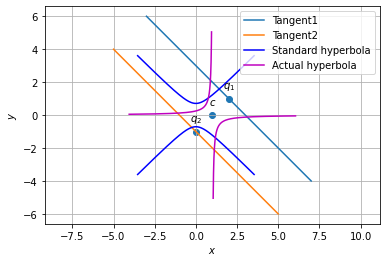
\includegraphics[width=\columnwidth]{./solutions/1/14/graph7.png}
	\caption{The standard and actual hyperbola.}
\end{figure}


\subsection{Lines and Plane }
\subsubsection{Problem}
\begin{flushleft}
Find the center and radius of the circle
\begin{align}
\vec{x}^T\vec{x} + \myvec{8\\10}\vec{x} - 8 = 0
\end{align}
\end{flushleft}

\subsubsection{Solution}
The given curve 
\begin{align}
	y =\frac{1}{x-1}
\end{align}
can be expressed as 
\begin{align}
	xy - y - 1 = 0 \label{eq:solutions/1/14/eq:hyperbola}
\end{align}
Hence, we have
\begin{align}
	\vec{V} = \frac{1}{2}\myvec{0 & 1 \\ 1 & 0}, 
	\vec{u} = \frac{1}{2}\myvec{0 \\-1},
	f = -1
\end{align}
Since $\mydet{\vec{V}} < 0$, the equation \eqref{eq:solutions/1/14/eq:hyperbola} represents hyperbola.
To find the values of $\lambda_1$ and $\lambda_2$, consider the characteristic equation,
\begin{align}
	\mydet{\lambda\vec{I} - \vec{V}} &= 0\\
	\implies \mydet{\myvec{\lambda & 0\\0 & \lambda} - \myvec{0 & \frac{1}{2} \\ \frac{1}{2} & 0}} &= 0\\
	\implies \mydet{ \lambda & \frac{-1}{2} \\ \frac{-1}{2} & \lambda} &= 0\\
	\implies \lambda_1 &= \frac{1}{2} , \lambda_2 = \frac{-1}{2}
\end{align}
In addition, given the slope -1, the direction and normal vectors are given by 
\begin{align}
	\vec{m} = \myvec{1 \\ -1} \\
	\vec{n} = \myvec{ 1 \\ 1}
\end{align}
The parameters of hyperbola are as follows:
\begin{align}
	\vec{c} &= -\vec{V}^{-1}\vec{u} \\
	&= -\myvec{0 & 2\\ 2 & 0}\myvec{0 \\ -\frac{1}{2}} \\
	&= \myvec{1 \\ 0}\\
	axes &= \begin{cases}
	\sqrt{\frac{\vec{u}^T\vec{V}^{-1}\vec{u} - f}{\lambda_1}} = \sqrt{2}\\
 \sqrt{\frac{f-\vec{u}^T\vec{V}^{-1}\vec{u}}{\lambda_2}} = \sqrt{2}
\end{cases}
\end{align}
which represents the standard hyperbola equation,
\begin{align}
	\frac{x^2}{2} - \frac{x^2}{2} = 1
\end{align}
The points of contact are given by 
\begin{align}
  \tiny{K} &=\pm \sqrt{\frac{\vec{u}^T\vec{V}^{-1}\vec{u} - f}{\vec{n}^T\vec{V}^{-1}\vec{n}}}
  = \pm \frac{1}{2}\\
  \vec{q} &= \vec{V}^{-1}(k\vec{n}-\vec{u})\\
  \vec{q_1} &= \myvec{0 & 2\\2 & 0} \sbrak{\frac{1}{2}\myvec{1 \\ 1} - \myvec{0\\ \frac{-1}{2}}}\\
  &= \myvec{2 \\ 1}\\
  \vec{q_2} &= \myvec{0 & 2\\2 & 0} \sbrak{\frac{-1}{2}\myvec{1 \\ 1} - \myvec{0\\ \frac{-1}{2}}}\\
  &= \myvec{0 \\ -1}
\end{align} 
$\therefore$ The tangents are given by
\begin{align}
	\myvec{1 & 1} \brak{\vec{x} - \myvec{2 \\ 1}} = 0 \\
	\myvec{1 & 1} \brak{\vec{x} - \myvec{0 \\ -1}} = 0
\end{align}
The desired equations of all lines having slope -1 that are tangents to the curve $\frac{1}{x-1}, x \neq 1$ are given by
\begin{align}
	\myvec{1 & 1}\vec{x} &= 3 \\
	\myvec{1 & 1}\vec{x} &= -1 
\end{align}
The above results are verified in the following figure.
\begin{figure}[h!] \label{eq:solutions/1/14/fig:tangents}
	\centering
	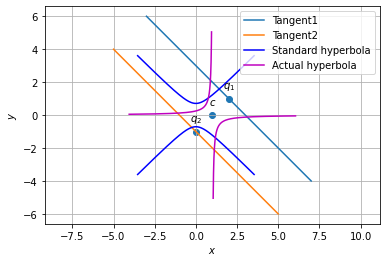
\includegraphics[width=\columnwidth]{./solutions/1/14/graph7.png}
	\caption{The standard and actual hyperbola.}
\end{figure}


\subsection{Motion in a Plane}
\subsubsection{Problem}
\begin{flushleft}
Find the center and radius of the circle
\begin{align}
\vec{x}^T\vec{x} + \myvec{8\\10}\vec{x} - 8 = 0
\end{align}
\end{flushleft}

\subsubsection{Solution}
The given curve 
\begin{align}
	y =\frac{1}{x-1}
\end{align}
can be expressed as 
\begin{align}
	xy - y - 1 = 0 \label{eq:solutions/1/14/eq:hyperbola}
\end{align}
Hence, we have
\begin{align}
	\vec{V} = \frac{1}{2}\myvec{0 & 1 \\ 1 & 0}, 
	\vec{u} = \frac{1}{2}\myvec{0 \\-1},
	f = -1
\end{align}
Since $\mydet{\vec{V}} < 0$, the equation \eqref{eq:solutions/1/14/eq:hyperbola} represents hyperbola.
To find the values of $\lambda_1$ and $\lambda_2$, consider the characteristic equation,
\begin{align}
	\mydet{\lambda\vec{I} - \vec{V}} &= 0\\
	\implies \mydet{\myvec{\lambda & 0\\0 & \lambda} - \myvec{0 & \frac{1}{2} \\ \frac{1}{2} & 0}} &= 0\\
	\implies \mydet{ \lambda & \frac{-1}{2} \\ \frac{-1}{2} & \lambda} &= 0\\
	\implies \lambda_1 &= \frac{1}{2} , \lambda_2 = \frac{-1}{2}
\end{align}
In addition, given the slope -1, the direction and normal vectors are given by 
\begin{align}
	\vec{m} = \myvec{1 \\ -1} \\
	\vec{n} = \myvec{ 1 \\ 1}
\end{align}
The parameters of hyperbola are as follows:
\begin{align}
	\vec{c} &= -\vec{V}^{-1}\vec{u} \\
	&= -\myvec{0 & 2\\ 2 & 0}\myvec{0 \\ -\frac{1}{2}} \\
	&= \myvec{1 \\ 0}\\
	axes &= \begin{cases}
	\sqrt{\frac{\vec{u}^T\vec{V}^{-1}\vec{u} - f}{\lambda_1}} = \sqrt{2}\\
 \sqrt{\frac{f-\vec{u}^T\vec{V}^{-1}\vec{u}}{\lambda_2}} = \sqrt{2}
\end{cases}
\end{align}
which represents the standard hyperbola equation,
\begin{align}
	\frac{x^2}{2} - \frac{x^2}{2} = 1
\end{align}
The points of contact are given by 
\begin{align}
  \tiny{K} &=\pm \sqrt{\frac{\vec{u}^T\vec{V}^{-1}\vec{u} - f}{\vec{n}^T\vec{V}^{-1}\vec{n}}}
  = \pm \frac{1}{2}\\
  \vec{q} &= \vec{V}^{-1}(k\vec{n}-\vec{u})\\
  \vec{q_1} &= \myvec{0 & 2\\2 & 0} \sbrak{\frac{1}{2}\myvec{1 \\ 1} - \myvec{0\\ \frac{-1}{2}}}\\
  &= \myvec{2 \\ 1}\\
  \vec{q_2} &= \myvec{0 & 2\\2 & 0} \sbrak{\frac{-1}{2}\myvec{1 \\ 1} - \myvec{0\\ \frac{-1}{2}}}\\
  &= \myvec{0 \\ -1}
\end{align} 
$\therefore$ The tangents are given by
\begin{align}
	\myvec{1 & 1} \brak{\vec{x} - \myvec{2 \\ 1}} = 0 \\
	\myvec{1 & 1} \brak{\vec{x} - \myvec{0 \\ -1}} = 0
\end{align}
The desired equations of all lines having slope -1 that are tangents to the curve $\frac{1}{x-1}, x \neq 1$ are given by
\begin{align}
	\myvec{1 & 1}\vec{x} &= 3 \\
	\myvec{1 & 1}\vec{x} &= -1 
\end{align}
The above results are verified in the following figure.
\begin{figure}[h!] \label{eq:solutions/1/14/fig:tangents}
	\centering
	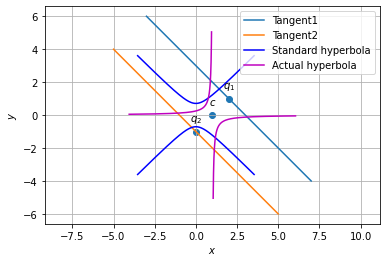
\includegraphics[width=\columnwidth]{./solutions/1/14/graph7.png}
	\caption{The standard and actual hyperbola.}
\end{figure}


\subsection{Determinants}
\subsubsection{Problem}
\begin{flushleft}
Find the center and radius of the circle
\begin{align}
\vec{x}^T\vec{x} + \myvec{8\\10}\vec{x} - 8 = 0
\end{align}
\end{flushleft}

\subsubsection{Solution}
The given curve 
\begin{align}
	y =\frac{1}{x-1}
\end{align}
can be expressed as 
\begin{align}
	xy - y - 1 = 0 \label{eq:solutions/1/14/eq:hyperbola}
\end{align}
Hence, we have
\begin{align}
	\vec{V} = \frac{1}{2}\myvec{0 & 1 \\ 1 & 0}, 
	\vec{u} = \frac{1}{2}\myvec{0 \\-1},
	f = -1
\end{align}
Since $\mydet{\vec{V}} < 0$, the equation \eqref{eq:solutions/1/14/eq:hyperbola} represents hyperbola.
To find the values of $\lambda_1$ and $\lambda_2$, consider the characteristic equation,
\begin{align}
	\mydet{\lambda\vec{I} - \vec{V}} &= 0\\
	\implies \mydet{\myvec{\lambda & 0\\0 & \lambda} - \myvec{0 & \frac{1}{2} \\ \frac{1}{2} & 0}} &= 0\\
	\implies \mydet{ \lambda & \frac{-1}{2} \\ \frac{-1}{2} & \lambda} &= 0\\
	\implies \lambda_1 &= \frac{1}{2} , \lambda_2 = \frac{-1}{2}
\end{align}
In addition, given the slope -1, the direction and normal vectors are given by 
\begin{align}
	\vec{m} = \myvec{1 \\ -1} \\
	\vec{n} = \myvec{ 1 \\ 1}
\end{align}
The parameters of hyperbola are as follows:
\begin{align}
	\vec{c} &= -\vec{V}^{-1}\vec{u} \\
	&= -\myvec{0 & 2\\ 2 & 0}\myvec{0 \\ -\frac{1}{2}} \\
	&= \myvec{1 \\ 0}\\
	axes &= \begin{cases}
	\sqrt{\frac{\vec{u}^T\vec{V}^{-1}\vec{u} - f}{\lambda_1}} = \sqrt{2}\\
 \sqrt{\frac{f-\vec{u}^T\vec{V}^{-1}\vec{u}}{\lambda_2}} = \sqrt{2}
\end{cases}
\end{align}
which represents the standard hyperbola equation,
\begin{align}
	\frac{x^2}{2} - \frac{x^2}{2} = 1
\end{align}
The points of contact are given by 
\begin{align}
  \tiny{K} &=\pm \sqrt{\frac{\vec{u}^T\vec{V}^{-1}\vec{u} - f}{\vec{n}^T\vec{V}^{-1}\vec{n}}}
  = \pm \frac{1}{2}\\
  \vec{q} &= \vec{V}^{-1}(k\vec{n}-\vec{u})\\
  \vec{q_1} &= \myvec{0 & 2\\2 & 0} \sbrak{\frac{1}{2}\myvec{1 \\ 1} - \myvec{0\\ \frac{-1}{2}}}\\
  &= \myvec{2 \\ 1}\\
  \vec{q_2} &= \myvec{0 & 2\\2 & 0} \sbrak{\frac{-1}{2}\myvec{1 \\ 1} - \myvec{0\\ \frac{-1}{2}}}\\
  &= \myvec{0 \\ -1}
\end{align} 
$\therefore$ The tangents are given by
\begin{align}
	\myvec{1 & 1} \brak{\vec{x} - \myvec{2 \\ 1}} = 0 \\
	\myvec{1 & 1} \brak{\vec{x} - \myvec{0 \\ -1}} = 0
\end{align}
The desired equations of all lines having slope -1 that are tangents to the curve $\frac{1}{x-1}, x \neq 1$ are given by
\begin{align}
	\myvec{1 & 1}\vec{x} &= 3 \\
	\myvec{1 & 1}\vec{x} &= -1 
\end{align}
The above results are verified in the following figure.
\begin{figure}[h!] \label{eq:solutions/1/14/fig:tangents}
	\centering
	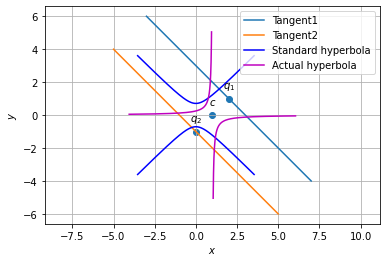
\includegraphics[width=\columnwidth]{./solutions/1/14/graph7.png}
	\caption{The standard and actual hyperbola.}
\end{figure}


\subsection{Linear Inequalities}
\subsubsection{Problem}
\begin{flushleft}
Find the center and radius of the circle
\begin{align}
\vec{x}^T\vec{x} + \myvec{8\\10}\vec{x} - 8 = 0
\end{align}
\end{flushleft}

\subsubsection{Solution}
The given curve 
\begin{align}
	y =\frac{1}{x-1}
\end{align}
can be expressed as 
\begin{align}
	xy - y - 1 = 0 \label{eq:solutions/1/14/eq:hyperbola}
\end{align}
Hence, we have
\begin{align}
	\vec{V} = \frac{1}{2}\myvec{0 & 1 \\ 1 & 0}, 
	\vec{u} = \frac{1}{2}\myvec{0 \\-1},
	f = -1
\end{align}
Since $\mydet{\vec{V}} < 0$, the equation \eqref{eq:solutions/1/14/eq:hyperbola} represents hyperbola.
To find the values of $\lambda_1$ and $\lambda_2$, consider the characteristic equation,
\begin{align}
	\mydet{\lambda\vec{I} - \vec{V}} &= 0\\
	\implies \mydet{\myvec{\lambda & 0\\0 & \lambda} - \myvec{0 & \frac{1}{2} \\ \frac{1}{2} & 0}} &= 0\\
	\implies \mydet{ \lambda & \frac{-1}{2} \\ \frac{-1}{2} & \lambda} &= 0\\
	\implies \lambda_1 &= \frac{1}{2} , \lambda_2 = \frac{-1}{2}
\end{align}
In addition, given the slope -1, the direction and normal vectors are given by 
\begin{align}
	\vec{m} = \myvec{1 \\ -1} \\
	\vec{n} = \myvec{ 1 \\ 1}
\end{align}
The parameters of hyperbola are as follows:
\begin{align}
	\vec{c} &= -\vec{V}^{-1}\vec{u} \\
	&= -\myvec{0 & 2\\ 2 & 0}\myvec{0 \\ -\frac{1}{2}} \\
	&= \myvec{1 \\ 0}\\
	axes &= \begin{cases}
	\sqrt{\frac{\vec{u}^T\vec{V}^{-1}\vec{u} - f}{\lambda_1}} = \sqrt{2}\\
 \sqrt{\frac{f-\vec{u}^T\vec{V}^{-1}\vec{u}}{\lambda_2}} = \sqrt{2}
\end{cases}
\end{align}
which represents the standard hyperbola equation,
\begin{align}
	\frac{x^2}{2} - \frac{x^2}{2} = 1
\end{align}
The points of contact are given by 
\begin{align}
  \tiny{K} &=\pm \sqrt{\frac{\vec{u}^T\vec{V}^{-1}\vec{u} - f}{\vec{n}^T\vec{V}^{-1}\vec{n}}}
  = \pm \frac{1}{2}\\
  \vec{q} &= \vec{V}^{-1}(k\vec{n}-\vec{u})\\
  \vec{q_1} &= \myvec{0 & 2\\2 & 0} \sbrak{\frac{1}{2}\myvec{1 \\ 1} - \myvec{0\\ \frac{-1}{2}}}\\
  &= \myvec{2 \\ 1}\\
  \vec{q_2} &= \myvec{0 & 2\\2 & 0} \sbrak{\frac{-1}{2}\myvec{1 \\ 1} - \myvec{0\\ \frac{-1}{2}}}\\
  &= \myvec{0 \\ -1}
\end{align} 
$\therefore$ The tangents are given by
\begin{align}
	\myvec{1 & 1} \brak{\vec{x} - \myvec{2 \\ 1}} = 0 \\
	\myvec{1 & 1} \brak{\vec{x} - \myvec{0 \\ -1}} = 0
\end{align}
The desired equations of all lines having slope -1 that are tangents to the curve $\frac{1}{x-1}, x \neq 1$ are given by
\begin{align}
	\myvec{1 & 1}\vec{x} &= 3 \\
	\myvec{1 & 1}\vec{x} &= -1 
\end{align}
The above results are verified in the following figure.
\begin{figure}[h!] \label{eq:solutions/1/14/fig:tangents}
	\centering
	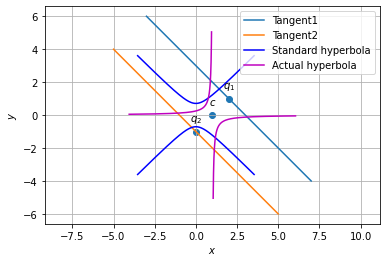
\includegraphics[width=\columnwidth]{./solutions/1/14/graph7.png}
	\caption{The standard and actual hyperbola.}
\end{figure}


\subsection{Miscellaneous}
\subsubsection{Problem}
\begin{flushleft}
Find the center and radius of the circle
\begin{align}
\vec{x}^T\vec{x} + \myvec{8\\10}\vec{x} - 8 = 0
\end{align}
\end{flushleft}

\subsubsection{Solution}
The given curve 
\begin{align}
	y =\frac{1}{x-1}
\end{align}
can be expressed as 
\begin{align}
	xy - y - 1 = 0 \label{eq:solutions/1/14/eq:hyperbola}
\end{align}
Hence, we have
\begin{align}
	\vec{V} = \frac{1}{2}\myvec{0 & 1 \\ 1 & 0}, 
	\vec{u} = \frac{1}{2}\myvec{0 \\-1},
	f = -1
\end{align}
Since $\mydet{\vec{V}} < 0$, the equation \eqref{eq:solutions/1/14/eq:hyperbola} represents hyperbola.
To find the values of $\lambda_1$ and $\lambda_2$, consider the characteristic equation,
\begin{align}
	\mydet{\lambda\vec{I} - \vec{V}} &= 0\\
	\implies \mydet{\myvec{\lambda & 0\\0 & \lambda} - \myvec{0 & \frac{1}{2} \\ \frac{1}{2} & 0}} &= 0\\
	\implies \mydet{ \lambda & \frac{-1}{2} \\ \frac{-1}{2} & \lambda} &= 0\\
	\implies \lambda_1 &= \frac{1}{2} , \lambda_2 = \frac{-1}{2}
\end{align}
In addition, given the slope -1, the direction and normal vectors are given by 
\begin{align}
	\vec{m} = \myvec{1 \\ -1} \\
	\vec{n} = \myvec{ 1 \\ 1}
\end{align}
The parameters of hyperbola are as follows:
\begin{align}
	\vec{c} &= -\vec{V}^{-1}\vec{u} \\
	&= -\myvec{0 & 2\\ 2 & 0}\myvec{0 \\ -\frac{1}{2}} \\
	&= \myvec{1 \\ 0}\\
	axes &= \begin{cases}
	\sqrt{\frac{\vec{u}^T\vec{V}^{-1}\vec{u} - f}{\lambda_1}} = \sqrt{2}\\
 \sqrt{\frac{f-\vec{u}^T\vec{V}^{-1}\vec{u}}{\lambda_2}} = \sqrt{2}
\end{cases}
\end{align}
which represents the standard hyperbola equation,
\begin{align}
	\frac{x^2}{2} - \frac{x^2}{2} = 1
\end{align}
The points of contact are given by 
\begin{align}
  \tiny{K} &=\pm \sqrt{\frac{\vec{u}^T\vec{V}^{-1}\vec{u} - f}{\vec{n}^T\vec{V}^{-1}\vec{n}}}
  = \pm \frac{1}{2}\\
  \vec{q} &= \vec{V}^{-1}(k\vec{n}-\vec{u})\\
  \vec{q_1} &= \myvec{0 & 2\\2 & 0} \sbrak{\frac{1}{2}\myvec{1 \\ 1} - \myvec{0\\ \frac{-1}{2}}}\\
  &= \myvec{2 \\ 1}\\
  \vec{q_2} &= \myvec{0 & 2\\2 & 0} \sbrak{\frac{-1}{2}\myvec{1 \\ 1} - \myvec{0\\ \frac{-1}{2}}}\\
  &= \myvec{0 \\ -1}
\end{align} 
$\therefore$ The tangents are given by
\begin{align}
	\myvec{1 & 1} \brak{\vec{x} - \myvec{2 \\ 1}} = 0 \\
	\myvec{1 & 1} \brak{\vec{x} - \myvec{0 \\ -1}} = 0
\end{align}
The desired equations of all lines having slope -1 that are tangents to the curve $\frac{1}{x-1}, x \neq 1$ are given by
\begin{align}
	\myvec{1 & 1}\vec{x} &= 3 \\
	\myvec{1 & 1}\vec{x} &= -1 
\end{align}
The above results are verified in the following figure.
\begin{figure}[h!] \label{eq:solutions/1/14/fig:tangents}
	\centering
	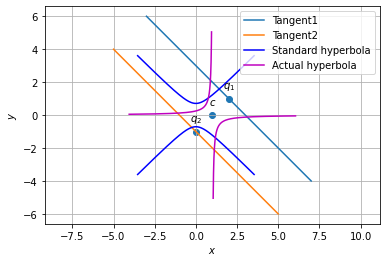
\includegraphics[width=\columnwidth]{./solutions/1/14/graph7.png}
	\caption{The standard and actual hyperbola.}
\end{figure}


\section{CIRCLE EXERCISE}
\subsection{Problem}
\begin{flushleft}
Find the center and radius of the circle
\begin{align}
\vec{x}^T\vec{x} + \myvec{8\\10}\vec{x} - 8 = 0
\end{align}
\end{flushleft}

\subsection{Solution}
The given curve 
\begin{align}
	y =\frac{1}{x-1}
\end{align}
can be expressed as 
\begin{align}
	xy - y - 1 = 0 \label{eq:solutions/1/14/eq:hyperbola}
\end{align}
Hence, we have
\begin{align}
	\vec{V} = \frac{1}{2}\myvec{0 & 1 \\ 1 & 0}, 
	\vec{u} = \frac{1}{2}\myvec{0 \\-1},
	f = -1
\end{align}
Since $\mydet{\vec{V}} < 0$, the equation \eqref{eq:solutions/1/14/eq:hyperbola} represents hyperbola.
To find the values of $\lambda_1$ and $\lambda_2$, consider the characteristic equation,
\begin{align}
	\mydet{\lambda\vec{I} - \vec{V}} &= 0\\
	\implies \mydet{\myvec{\lambda & 0\\0 & \lambda} - \myvec{0 & \frac{1}{2} \\ \frac{1}{2} & 0}} &= 0\\
	\implies \mydet{ \lambda & \frac{-1}{2} \\ \frac{-1}{2} & \lambda} &= 0\\
	\implies \lambda_1 &= \frac{1}{2} , \lambda_2 = \frac{-1}{2}
\end{align}
In addition, given the slope -1, the direction and normal vectors are given by 
\begin{align}
	\vec{m} = \myvec{1 \\ -1} \\
	\vec{n} = \myvec{ 1 \\ 1}
\end{align}
The parameters of hyperbola are as follows:
\begin{align}
	\vec{c} &= -\vec{V}^{-1}\vec{u} \\
	&= -\myvec{0 & 2\\ 2 & 0}\myvec{0 \\ -\frac{1}{2}} \\
	&= \myvec{1 \\ 0}\\
	axes &= \begin{cases}
	\sqrt{\frac{\vec{u}^T\vec{V}^{-1}\vec{u} - f}{\lambda_1}} = \sqrt{2}\\
 \sqrt{\frac{f-\vec{u}^T\vec{V}^{-1}\vec{u}}{\lambda_2}} = \sqrt{2}
\end{cases}
\end{align}
which represents the standard hyperbola equation,
\begin{align}
	\frac{x^2}{2} - \frac{x^2}{2} = 1
\end{align}
The points of contact are given by 
\begin{align}
  \tiny{K} &=\pm \sqrt{\frac{\vec{u}^T\vec{V}^{-1}\vec{u} - f}{\vec{n}^T\vec{V}^{-1}\vec{n}}}
  = \pm \frac{1}{2}\\
  \vec{q} &= \vec{V}^{-1}(k\vec{n}-\vec{u})\\
  \vec{q_1} &= \myvec{0 & 2\\2 & 0} \sbrak{\frac{1}{2}\myvec{1 \\ 1} - \myvec{0\\ \frac{-1}{2}}}\\
  &= \myvec{2 \\ 1}\\
  \vec{q_2} &= \myvec{0 & 2\\2 & 0} \sbrak{\frac{-1}{2}\myvec{1 \\ 1} - \myvec{0\\ \frac{-1}{2}}}\\
  &= \myvec{0 \\ -1}
\end{align} 
$\therefore$ The tangents are given by
\begin{align}
	\myvec{1 & 1} \brak{\vec{x} - \myvec{2 \\ 1}} = 0 \\
	\myvec{1 & 1} \brak{\vec{x} - \myvec{0 \\ -1}} = 0
\end{align}
The desired equations of all lines having slope -1 that are tangents to the curve $\frac{1}{x-1}, x \neq 1$ are given by
\begin{align}
	\myvec{1 & 1}\vec{x} &= 3 \\
	\myvec{1 & 1}\vec{x} &= -1 
\end{align}
The above results are verified in the following figure.
\begin{figure}[h!] \label{eq:solutions/1/14/fig:tangents}
	\centering
	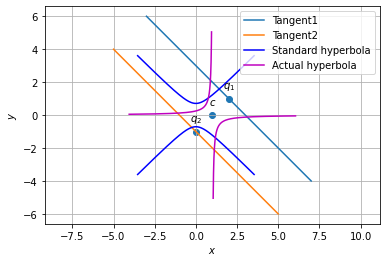
\includegraphics[width=\columnwidth]{./solutions/1/14/graph7.png}
	\caption{The standard and actual hyperbola.}
\end{figure}


\section{CONICS EXERCISE}
\subsection{Problem}
\begin{flushleft}
Find the center and radius of the circle
\begin{align}
\vec{x}^T\vec{x} + \myvec{8\\10}\vec{x} - 8 = 0
\end{align}
\end{flushleft}

\subsection{Solution}
The given curve 
\begin{align}
	y =\frac{1}{x-1}
\end{align}
can be expressed as 
\begin{align}
	xy - y - 1 = 0 \label{eq:solutions/1/14/eq:hyperbola}
\end{align}
Hence, we have
\begin{align}
	\vec{V} = \frac{1}{2}\myvec{0 & 1 \\ 1 & 0}, 
	\vec{u} = \frac{1}{2}\myvec{0 \\-1},
	f = -1
\end{align}
Since $\mydet{\vec{V}} < 0$, the equation \eqref{eq:solutions/1/14/eq:hyperbola} represents hyperbola.
To find the values of $\lambda_1$ and $\lambda_2$, consider the characteristic equation,
\begin{align}
	\mydet{\lambda\vec{I} - \vec{V}} &= 0\\
	\implies \mydet{\myvec{\lambda & 0\\0 & \lambda} - \myvec{0 & \frac{1}{2} \\ \frac{1}{2} & 0}} &= 0\\
	\implies \mydet{ \lambda & \frac{-1}{2} \\ \frac{-1}{2} & \lambda} &= 0\\
	\implies \lambda_1 &= \frac{1}{2} , \lambda_2 = \frac{-1}{2}
\end{align}
In addition, given the slope -1, the direction and normal vectors are given by 
\begin{align}
	\vec{m} = \myvec{1 \\ -1} \\
	\vec{n} = \myvec{ 1 \\ 1}
\end{align}
The parameters of hyperbola are as follows:
\begin{align}
	\vec{c} &= -\vec{V}^{-1}\vec{u} \\
	&= -\myvec{0 & 2\\ 2 & 0}\myvec{0 \\ -\frac{1}{2}} \\
	&= \myvec{1 \\ 0}\\
	axes &= \begin{cases}
	\sqrt{\frac{\vec{u}^T\vec{V}^{-1}\vec{u} - f}{\lambda_1}} = \sqrt{2}\\
 \sqrt{\frac{f-\vec{u}^T\vec{V}^{-1}\vec{u}}{\lambda_2}} = \sqrt{2}
\end{cases}
\end{align}
which represents the standard hyperbola equation,
\begin{align}
	\frac{x^2}{2} - \frac{x^2}{2} = 1
\end{align}
The points of contact are given by 
\begin{align}
  \tiny{K} &=\pm \sqrt{\frac{\vec{u}^T\vec{V}^{-1}\vec{u} - f}{\vec{n}^T\vec{V}^{-1}\vec{n}}}
  = \pm \frac{1}{2}\\
  \vec{q} &= \vec{V}^{-1}(k\vec{n}-\vec{u})\\
  \vec{q_1} &= \myvec{0 & 2\\2 & 0} \sbrak{\frac{1}{2}\myvec{1 \\ 1} - \myvec{0\\ \frac{-1}{2}}}\\
  &= \myvec{2 \\ 1}\\
  \vec{q_2} &= \myvec{0 & 2\\2 & 0} \sbrak{\frac{-1}{2}\myvec{1 \\ 1} - \myvec{0\\ \frac{-1}{2}}}\\
  &= \myvec{0 \\ -1}
\end{align} 
$\therefore$ The tangents are given by
\begin{align}
	\myvec{1 & 1} \brak{\vec{x} - \myvec{2 \\ 1}} = 0 \\
	\myvec{1 & 1} \brak{\vec{x} - \myvec{0 \\ -1}} = 0
\end{align}
The desired equations of all lines having slope -1 that are tangents to the curve $\frac{1}{x-1}, x \neq 1$ are given by
\begin{align}
	\myvec{1 & 1}\vec{x} &= 3 \\
	\myvec{1 & 1}\vec{x} &= -1 
\end{align}
The above results are verified in the following figure.
\begin{figure}[h!] \label{eq:solutions/1/14/fig:tangents}
	\centering
	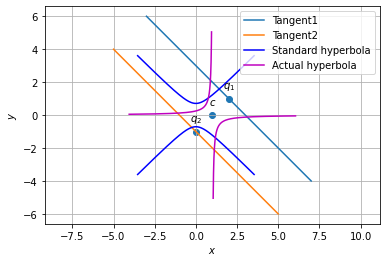
\includegraphics[width=\columnwidth]{./solutions/1/14/graph7.png}
	\caption{The standard and actual hyperbola.}
\end{figure}


\end{document}

